\documentclass[border=6pt]{standalone}
\usepackage{pgfplots}
\pgfplotsset{compat=1.18}
\usepackage{xcolor}
\definecolor{fam0}{HTML}{2A78D6}
\definecolor{fam1}{HTML}{EB6834}
\definecolor{fam2}{HTML}{1BAF7A}
\definecolor{fam3}{HTML}{4A3AA7}
\definecolor{fam4}{HTML}{0B0B0B}
\definecolor{surface}{HTML}{FCFCFB}
\definecolor{ink}{HTML}{0B0B0B}
\definecolor{muted}{HTML}{52514E}
\definecolor{gridc}{HTML}{E8E7E3}
\begin{document}
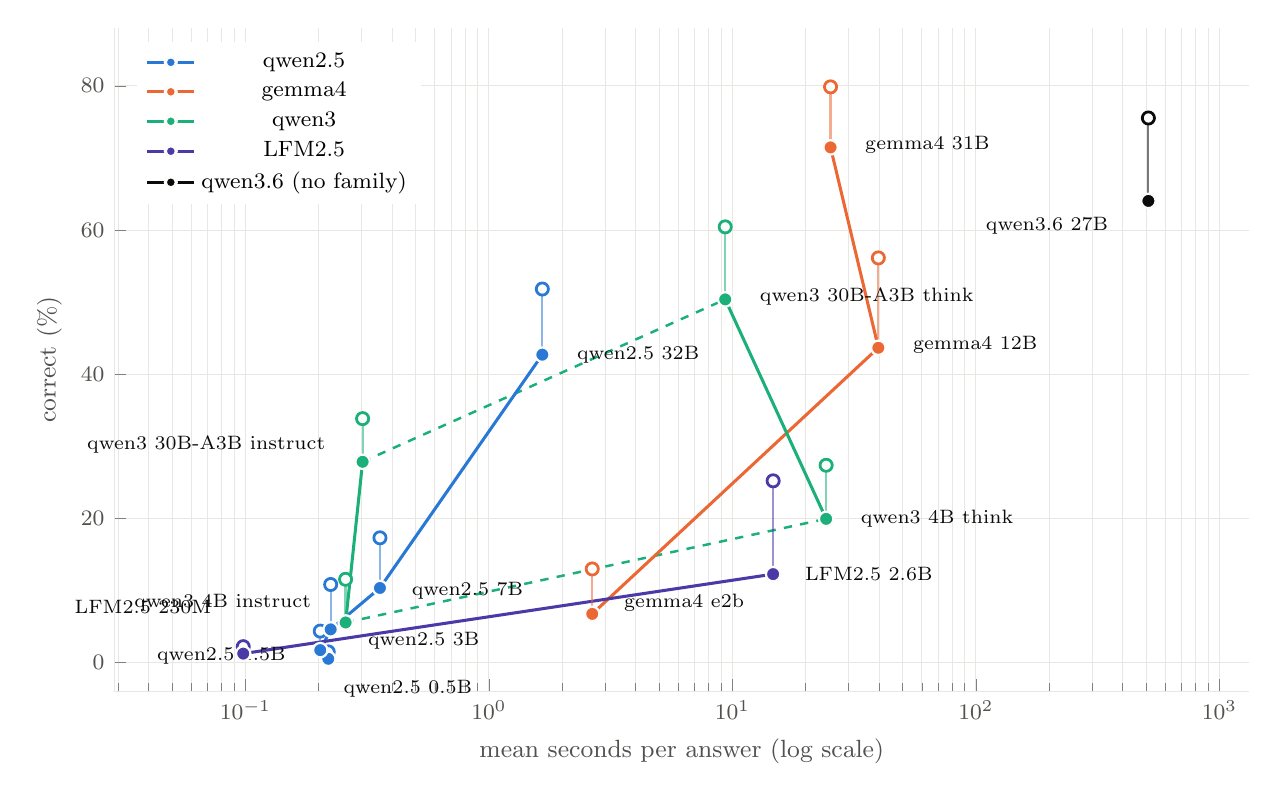
\begin{tikzpicture}
\begin{axis}[
  width=16cm, height=10cm, xmode=log, log basis x=10,
  xlabel={mean seconds per answer (log scale)},
  ylabel={correct (\%)},
  xlabel style={font=\small, color=muted},
  ylabel style={font=\small, color=muted},
  tick label style={font=\footnotesize, color=muted},
  ymin=-4, ymax=88, xmin=0.0289, xmax=1328.8,
  grid=both, grid style={gridc, line width=0.3pt},
  axis line style={gridc}, axis x line*=bottom, axis y line*=left,
  clip=false, legend style={draw=none, font=\footnotesize, at={(0.02,0.98)}, anchor=north west},
]
% instruct -> thinking
\addplot[fam2, dashed, line width=0.9pt, forget plot] coordinates {(0.258,5.52) (24.276,19.90)};
\addplot[fam2, dashed, line width=0.9pt, forget plot] coordinates {(0.303,27.82) (9.347,50.36)};
% scale ladders
\addplot[fam0, line width=1.1pt, forget plot] coordinates {(0.219,0.48) (0.203,1.68) (0.224,4.56) (0.357,10.31) (1.658,42.69)};
\addplot[fam1, line width=1.1pt, forget plot] coordinates {(2.658,6.71) (39.779,43.65) (25.309,71.46)};
\addplot[fam3, line width=1.1pt, forget plot] coordinates {(0.098,1.20) (14.705,12.23)};
\addplot[fam2, line width=1.1pt, forget plot] coordinates {(0.258,5.52) (0.303,27.82)};
\addplot[fam2, line width=1.1pt, forget plot] coordinates {(24.276,19.90) (9.347,50.36)};
% pass@1 -> pass@3 stems
\addplot[fam3, opacity=0.55, line width=0.8pt, forget plot] coordinates {(14.705,12.23) (14.705,25.18)};
\addplot[fam3, opacity=0.55, line width=0.8pt, forget plot] coordinates {(0.098,1.20) (0.098,2.16)};
\addplot[fam0, opacity=0.55, line width=0.8pt, forget plot] coordinates {(0.219,0.48) (0.219,1.44)};
\addplot[fam0, opacity=0.55, line width=0.8pt, forget plot] coordinates {(0.203,1.68) (0.203,4.32)};
\addplot[fam0, opacity=0.55, line width=0.8pt, forget plot] coordinates {(0.224,4.56) (0.224,10.79)};
\addplot[fam0, opacity=0.55, line width=0.8pt, forget plot] coordinates {(0.357,10.31) (0.357,17.27)};
\addplot[fam0, opacity=0.55, line width=0.8pt, forget plot] coordinates {(1.658,42.69) (1.658,51.80)};
\addplot[fam1, opacity=0.55, line width=0.8pt, forget plot] coordinates {(2.658,6.71) (2.658,12.95)};
\addplot[fam1, opacity=0.55, line width=0.8pt, forget plot] coordinates {(39.779,43.65) (39.779,56.12)};
\addplot[fam1, opacity=0.55, line width=0.8pt, forget plot] coordinates {(25.309,71.46) (25.309,79.86)};
\addplot[fam2, opacity=0.55, line width=0.8pt, forget plot] coordinates {(24.276,19.90) (24.276,27.34)};
\addplot[fam2, opacity=0.55, line width=0.8pt, forget plot] coordinates {(0.258,5.52) (0.258,11.51)};
\addplot[fam2, opacity=0.55, line width=0.8pt, forget plot] coordinates {(9.347,50.36) (9.347,60.43)};
\addplot[fam2, opacity=0.55, line width=0.8pt, forget plot] coordinates {(0.303,27.82) (0.303,33.81)};
\addplot[fam4, opacity=0.55, line width=0.8pt, forget plot] coordinates {(511.065,64.03) (511.065,75.54)};
% markers
\addplot[only marks, mark=*, mark size=2.2pt, mark options={fill=surface, draw=fam3, line width=1pt}, forget plot] coordinates {(14.705,25.18)};
\addplot[only marks, mark=*, mark size=2.6pt, mark options={fill=fam3, draw=surface, line width=0.8pt}, forget plot] coordinates {(14.705,12.23)};
\addplot[only marks, mark=*, mark size=2.2pt, mark options={fill=surface, draw=fam3, line width=1pt}, forget plot] coordinates {(0.098,2.16)};
\addplot[only marks, mark=*, mark size=2.6pt, mark options={fill=fam3, draw=surface, line width=0.8pt}, forget plot] coordinates {(0.098,1.20)};
\addplot[only marks, mark=*, mark size=2.2pt, mark options={fill=surface, draw=fam0, line width=1pt}, forget plot] coordinates {(0.219,1.44)};
\addplot[only marks, mark=*, mark size=2.6pt, mark options={fill=fam0, draw=surface, line width=0.8pt}, forget plot] coordinates {(0.219,0.48)};
\addplot[only marks, mark=*, mark size=2.2pt, mark options={fill=surface, draw=fam0, line width=1pt}, forget plot] coordinates {(0.203,4.32)};
\addplot[only marks, mark=*, mark size=2.6pt, mark options={fill=fam0, draw=surface, line width=0.8pt}, forget plot] coordinates {(0.203,1.68)};
\addplot[only marks, mark=*, mark size=2.2pt, mark options={fill=surface, draw=fam0, line width=1pt}, forget plot] coordinates {(0.224,10.79)};
\addplot[only marks, mark=*, mark size=2.6pt, mark options={fill=fam0, draw=surface, line width=0.8pt}, forget plot] coordinates {(0.224,4.56)};
\addplot[only marks, mark=*, mark size=2.2pt, mark options={fill=surface, draw=fam0, line width=1pt}, forget plot] coordinates {(0.357,17.27)};
\addplot[only marks, mark=*, mark size=2.6pt, mark options={fill=fam0, draw=surface, line width=0.8pt}, forget plot] coordinates {(0.357,10.31)};
\addplot[only marks, mark=*, mark size=2.2pt, mark options={fill=surface, draw=fam0, line width=1pt}, forget plot] coordinates {(1.658,51.80)};
\addplot[only marks, mark=*, mark size=2.6pt, mark options={fill=fam0, draw=surface, line width=0.8pt}, forget plot] coordinates {(1.658,42.69)};
\addplot[only marks, mark=*, mark size=2.2pt, mark options={fill=surface, draw=fam1, line width=1pt}, forget plot] coordinates {(2.658,12.95)};
\addplot[only marks, mark=*, mark size=2.6pt, mark options={fill=fam1, draw=surface, line width=0.8pt}, forget plot] coordinates {(2.658,6.71)};
\addplot[only marks, mark=*, mark size=2.2pt, mark options={fill=surface, draw=fam1, line width=1pt}, forget plot] coordinates {(39.779,56.12)};
\addplot[only marks, mark=*, mark size=2.6pt, mark options={fill=fam1, draw=surface, line width=0.8pt}, forget plot] coordinates {(39.779,43.65)};
\addplot[only marks, mark=*, mark size=2.2pt, mark options={fill=surface, draw=fam1, line width=1pt}, forget plot] coordinates {(25.309,79.86)};
\addplot[only marks, mark=*, mark size=2.6pt, mark options={fill=fam1, draw=surface, line width=0.8pt}, forget plot] coordinates {(25.309,71.46)};
\addplot[only marks, mark=*, mark size=2.2pt, mark options={fill=surface, draw=fam2, line width=1pt}, forget plot] coordinates {(24.276,27.34)};
\addplot[only marks, mark=*, mark size=2.6pt, mark options={fill=fam2, draw=surface, line width=0.8pt}, forget plot] coordinates {(24.276,19.90)};
\addplot[only marks, mark=*, mark size=2.2pt, mark options={fill=surface, draw=fam2, line width=1pt}, forget plot] coordinates {(0.258,11.51)};
\addplot[only marks, mark=*, mark size=2.6pt, mark options={fill=fam2, draw=surface, line width=0.8pt}, forget plot] coordinates {(0.258,5.52)};
\addplot[only marks, mark=*, mark size=2.2pt, mark options={fill=surface, draw=fam2, line width=1pt}, forget plot] coordinates {(9.347,60.43)};
\addplot[only marks, mark=*, mark size=2.6pt, mark options={fill=fam2, draw=surface, line width=0.8pt}, forget plot] coordinates {(9.347,50.36)};
\addplot[only marks, mark=*, mark size=2.2pt, mark options={fill=surface, draw=fam2, line width=1pt}, forget plot] coordinates {(0.303,33.81)};
\addplot[only marks, mark=*, mark size=2.6pt, mark options={fill=fam2, draw=surface, line width=0.8pt}, forget plot] coordinates {(0.303,27.82)};
\addplot[only marks, mark=*, mark size=2.2pt, mark options={fill=surface, draw=fam4, line width=1pt}, forget plot] coordinates {(511.065,75.54)};
\addplot[only marks, mark=*, mark size=2.6pt, mark options={fill=fam4, draw=surface, line width=0.8pt}, forget plot] coordinates {(511.065,64.03)};
% labels
\node[anchor=west, font=\scriptsize, text=ink, xshift=8pt, yshift=0pt] at (axis cs:14.705,12.23) {LFM2.5 2.6B};
\node[anchor=east, font=\scriptsize, text=ink, xshift=-8pt, yshift=17pt] at (axis cs:0.098,1.20) {LFM2.5 230M};
\node[anchor=west, font=\scriptsize, text=ink, xshift=2pt, yshift=-11pt] at (axis cs:0.219,0.48) {qwen2.5 0.5B};
\node[anchor=east, font=\scriptsize, text=ink, xshift=-9pt, yshift=-2pt] at (axis cs:0.203,1.68) {qwen2.5 1.5B};
\node[anchor=west, font=\scriptsize, text=ink, xshift=10pt, yshift=-4pt] at (axis cs:0.224,4.56) {qwen2.5 3B};
\node[anchor=west, font=\scriptsize, text=ink, xshift=8pt, yshift=-1pt] at (axis cs:0.357,10.31) {qwen2.5 7B};
\node[anchor=west, font=\scriptsize, text=ink, xshift=9pt, yshift=0pt] at (axis cs:1.658,42.69) {qwen2.5 32B};
\node[anchor=west, font=\scriptsize, text=ink, xshift=8pt, yshift=4pt] at (axis cs:2.658,6.71) {gemma4 e2b};
\node[anchor=west, font=\scriptsize, text=ink, xshift=9pt, yshift=1pt] at (axis cs:39.779,43.65) {gemma4 12B};
\node[anchor=west, font=\scriptsize, text=ink, xshift=9pt, yshift=1pt] at (axis cs:25.309,71.46) {gemma4 31B};
\node[anchor=west, font=\scriptsize, text=ink, xshift=9pt, yshift=0pt] at (axis cs:24.276,19.90) {qwen3 4B think};
\node[anchor=east, font=\scriptsize, text=ink, xshift=-9pt, yshift=7pt] at (axis cs:0.258,5.52) {qwen3 4B instruct};
\node[anchor=west, font=\scriptsize, text=ink, xshift=9pt, yshift=1pt] at (axis cs:9.347,50.36) {qwen3 30B-A3B think};
\node[anchor=east, font=\scriptsize, text=ink, xshift=-10pt, yshift=6pt] at (axis cs:0.303,27.82) {qwen3 30B-A3B instruct};
\node[anchor=east, font=\scriptsize, text=ink, xshift=-11pt, yshift=-9pt] at (axis cs:511.065,64.03) {qwen3.6 27B};
\addlegendimage{fam0, line width=1.1pt, mark=*, mark options={fill=fam0, draw=surface}}
\addlegendentry{qwen2.5}
\addlegendimage{fam1, line width=1.1pt, mark=*, mark options={fill=fam1, draw=surface}}
\addlegendentry{gemma4}
\addlegendimage{fam2, line width=1.1pt, mark=*, mark options={fill=fam2, draw=surface}}
\addlegendentry{qwen3}
\addlegendimage{fam3, line width=1.1pt, mark=*, mark options={fill=fam3, draw=surface}}
\addlegendentry{LFM2.5}
\addlegendimage{fam4, line width=1.1pt, mark=*, mark options={fill=fam4, draw=surface}}
\addlegendentry{qwen3.6 (no family)}
\end{axis}
\end{tikzpicture}
\end{document}
